\chapter[Problema 01]{Problema 01}

Este capítulo discorrerá sobre o funcionamento de alguns protocolos utilizando uma ferramenta
de captura de pacotes selecionada. Ele conterá quatro tópicos, onde são mencionados os protocolos
HTTP, FTP e DNS, bem como a configuração da ferramenta. Não haverá um capítulo exclusivo para
TCP ou UDP pois estes serão explicados nos capítulos já mencionados.

\section{Configuração do Capturador de Pacotes}

O analisador de pacotes escolhido foi o Wireshark, pois este traz uma facilidade para a visualização
dos pacotes.
Para instalá-lo, foram utilizados os passos citados por \cite{instalacaowireshark}

Este ao ser iniciado solicita a interface de rede desejada, onde para cada problema, uma interface diferente
foi escolhida: Wlan, Lan, Loopback, etc.

\section{Protocolo HTTP}

\subsection{Configuração do Ambiente para a captura de pacotes utilizando protocolo HTTP}
A captura de pacotes foi procedida no Sistema operacional Linux kali 3.18.0 - kali 3 - amd64
Debian 3.18.6 - 1 GNU Linux.

O servidor HTTP foi ativado através da biblioteca SimpleHTTPServer nativa do python 2.7.3.
  A aplicação servidora foi iniciada no endereço de IP 127.0.0.1, na porta 8000.

O python é instalado por padrão em sistemas operacionais Linux. Dessa forma, para iniciar o
servidor no IP e porta mencionados deve-se utilizar o comando:

python -m SimpleHTTPServer 8000

A ferramenta de captura utilizada foi Wireshark, nativa no sistema operacional utilizado.
Este foi iniciado e configurado para analisar os pacotes da interface Loopback: lo.


\begin{itemize}

    \item Protocolo de Transporte Utilizado: TCP

    \item Endereço de IP e porta do Cliente: localhost: 47766

    \item Endereço de IP e porta do Servidor: localhost: 8000

\end{itemize}

\subsection{Capturas de Estabelecimento}
Como podemos observar na Figura \ref{fig:http} , o primeiro pacote da transação entre Cliente e Servidor é o
pedido de SYN do Cliente, mais conhecido como primeiro passo do three way handshake. O número de
  sequência deste é o 0 (Zero).

  \begin{figure}[h]
    \centering

    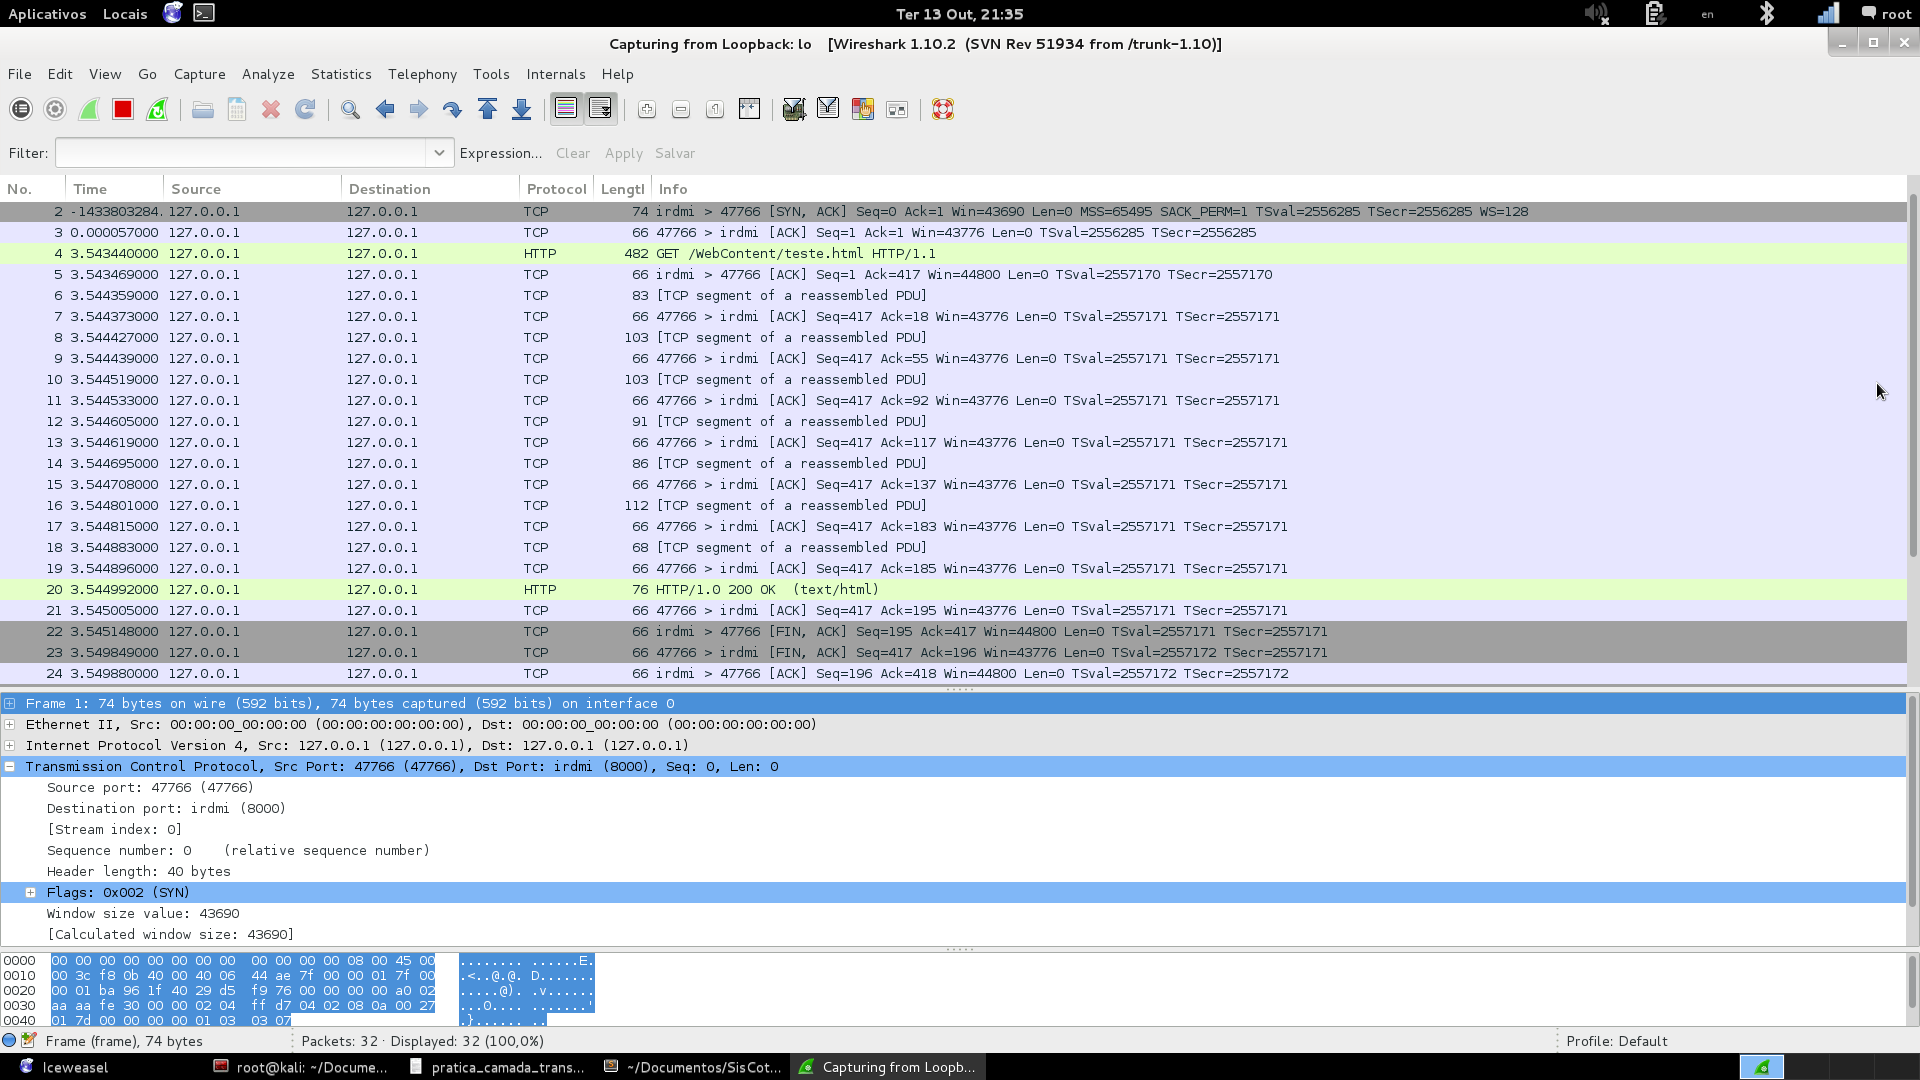
\includegraphics[width=450px, scale=1]{figuras/http}
    \caption{Capturas de Pacotes em uma transação HTTP}

 \label{fig:http}
  \end{figure}

O segundo pacote é uma resposta do servidor ao cliente, onde ele envia um ACK (acknowledgment)
para o Cliente, confirmando o seu pedido de sincronização. O seu numero de Ack é o 1, confirmando
que recebeu o número de sequência 0 do cliente e solicitando seu sucessor, o Seq = 1. Ao mesmo tempo,
  o servidor envia um SYN para o cliente com o objetivo de confirmar que está disponível para
  estabelecer uma conexão.

O terceiro e último passo do three way handshake é a confirmação da conexão do cliente para com o
servidor, ao enviar um ACK para o pedido de SYN.

Logo  após a execução do three way handshake e a conexão estabelecida, o cliente envia a sua
  requisição de página com o método GET. Este envia a mensagem com o cabeçalho especificando
  o que deseja do servidor:

Message: GET /WebContent/teste.html HTTP/ 1.1


\subsection{Capturas de Encerramento}
Logo após receber a mensagem do servidor contendo a confirmação com código 200 de Ok, a
conexão pode ser encerrada. Esse processo é iniciado quando o cliente envia um ACK, com
número de Seq=417, para o servidor quando recebe o payload da requisição executada.

Logo quando este chega ao servidor, ele envia uma flag FIN, com Seq = 195, sinalizando o
  início da conversa para finalizar a conexão e um ACK = 417, sinalizando que recebeu o
  último pacote do cliente.

O cliente responde o servidor, confirmando o seu pedido de finalização com ACK = 196 e
também executa o pedido de FIN, com seq = 417.

Terminando a conexão, o servidor emitiu a confirmação do pedido de finalização com o ACK = 418.


\section{Protocolo FTP}
\subsection{Configuração do Ambiente para a captura de pacotes utilizando protocolo FTP}
A captura de pacotes foi procedida no Sistema operacional Linux kali 3.18.0 - kali 3 - amd64
Debian 3.18.6 - 1 GNU Linux.

Para iniciar o servidor FTP, foi utilizada a ferramenta Vsftpd \cite{vsftpd} provê um servidor FTP no
endereço de IP desejado. Esta foi instalada e configurada de acordo com os passos mencionados por
\cite{instalacaovsftpd} .

Dessa maneira, a aplicação FTP foi iniciada na porta 21 da interface de rede Loopback.

A ferramenta de captura utilizada foi Wireshark, nativa no sistema operacional utilizado. Este foi iniciado e configurado para analisar os pacotes da interface Loopback: lo.


\begin{itemize}

    \item Protocolo de Transporte Utilizado: TCP

    \item Endereço de IP e porta do Cliente: localhost: 56909

    \item Endereço de IP e porta do Servidor: localhost: 21(FTP)

\end{itemize}

\subsection{Capturas de Estabelecimento}

Como podemos observar na figura \ref{fig:ftp1}, o primeiro pacote da transação entre Cliente e Servidor é
o pedido de SYN do Cliente, mais conhecido como primeiro passo do three way handshake. O
número de sequência deste é o 0 (Zero).

\begin{figure}[h]
  \centering

  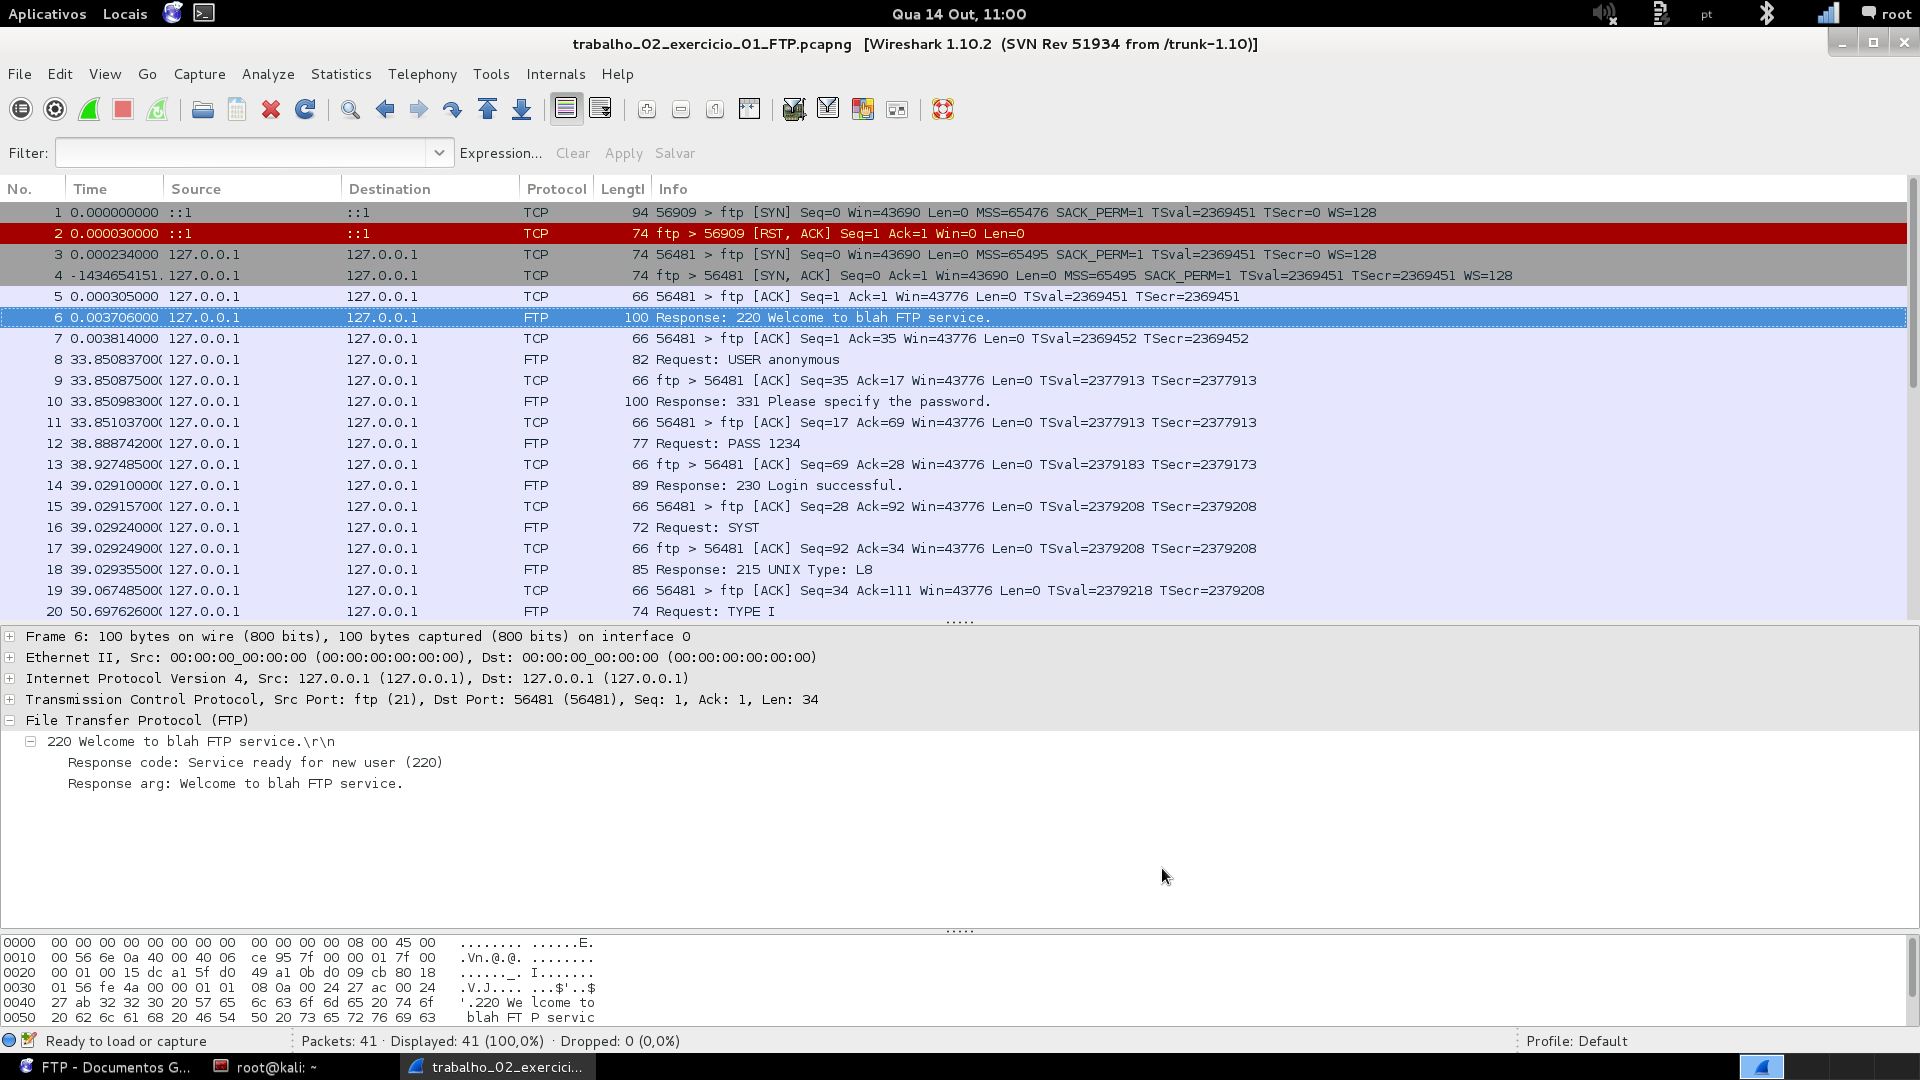
\includegraphics[width=450px, scale=1]{figuras/ftp1}
  \caption{Tree way handshake entre Cliente e Servidor}

\label{fig:ftp1}
\end{figure}

O segundo pacote é uma resposta do servidor ao cliente, onde ele envia um ACK (acknowledgment)
para o Cliente, confirmando o seu pedido de sincronização. O seu numero de Ack é o 1, confirmando que recebeu o número de sequência 0 do cliente e solicitando seu sucessor, o Seq = 1. Ao mesmo
tempo, o servidor envia um SYN para o cliente com o objetivo de confirmar que está disponível
 para estabelecer uma conexão.

O terceiro e último passo do three way handshake é a confirmação da conexão do cliente para
com o servidor, ao enviar um ACK para o pedido de SYN.

Logo  após a execução do three way handshake e a conexão estabelecida, o servidor envia uma
confirmação da conexão enviando o código 220 e a mensagem “Welcome to blah FTP service.”, que
foi pré configurada no servidor FTP. Além disso, o servidor solicita que o cliente informe o
 usuário que deseja utilizar para o acesso. Como a aplicação foi configurada para possibilitar
  acesso a qualquer usuário, este vai utilizar o usuário “anonymous” e assim pode entrar no
  sistema com qualquer senha.

O cliente informa o login solicitado com o campo preenchido com seu username:

Servidor responde com a solicitação de uma senha com uma mensagem no payload da camada de
aplicação: “Please specify the password.”

O cliente informa e envia o password, pode-se observar que o protocolo FTP possibilita
 a visualização do payload com o valor da senha informada, neste caso: 1234.


Por último, o login é aceito com sucesso.

Assim, o cliente executa um pedido de um arquivo contido na porta FTP do servidor da
 aplicação. Para isso, ele utilizou o comando get nomeDoArquivo.extensao. Neste cado o
  comando foi: get teste.html.

\begin{figure}[h]
  \centering

  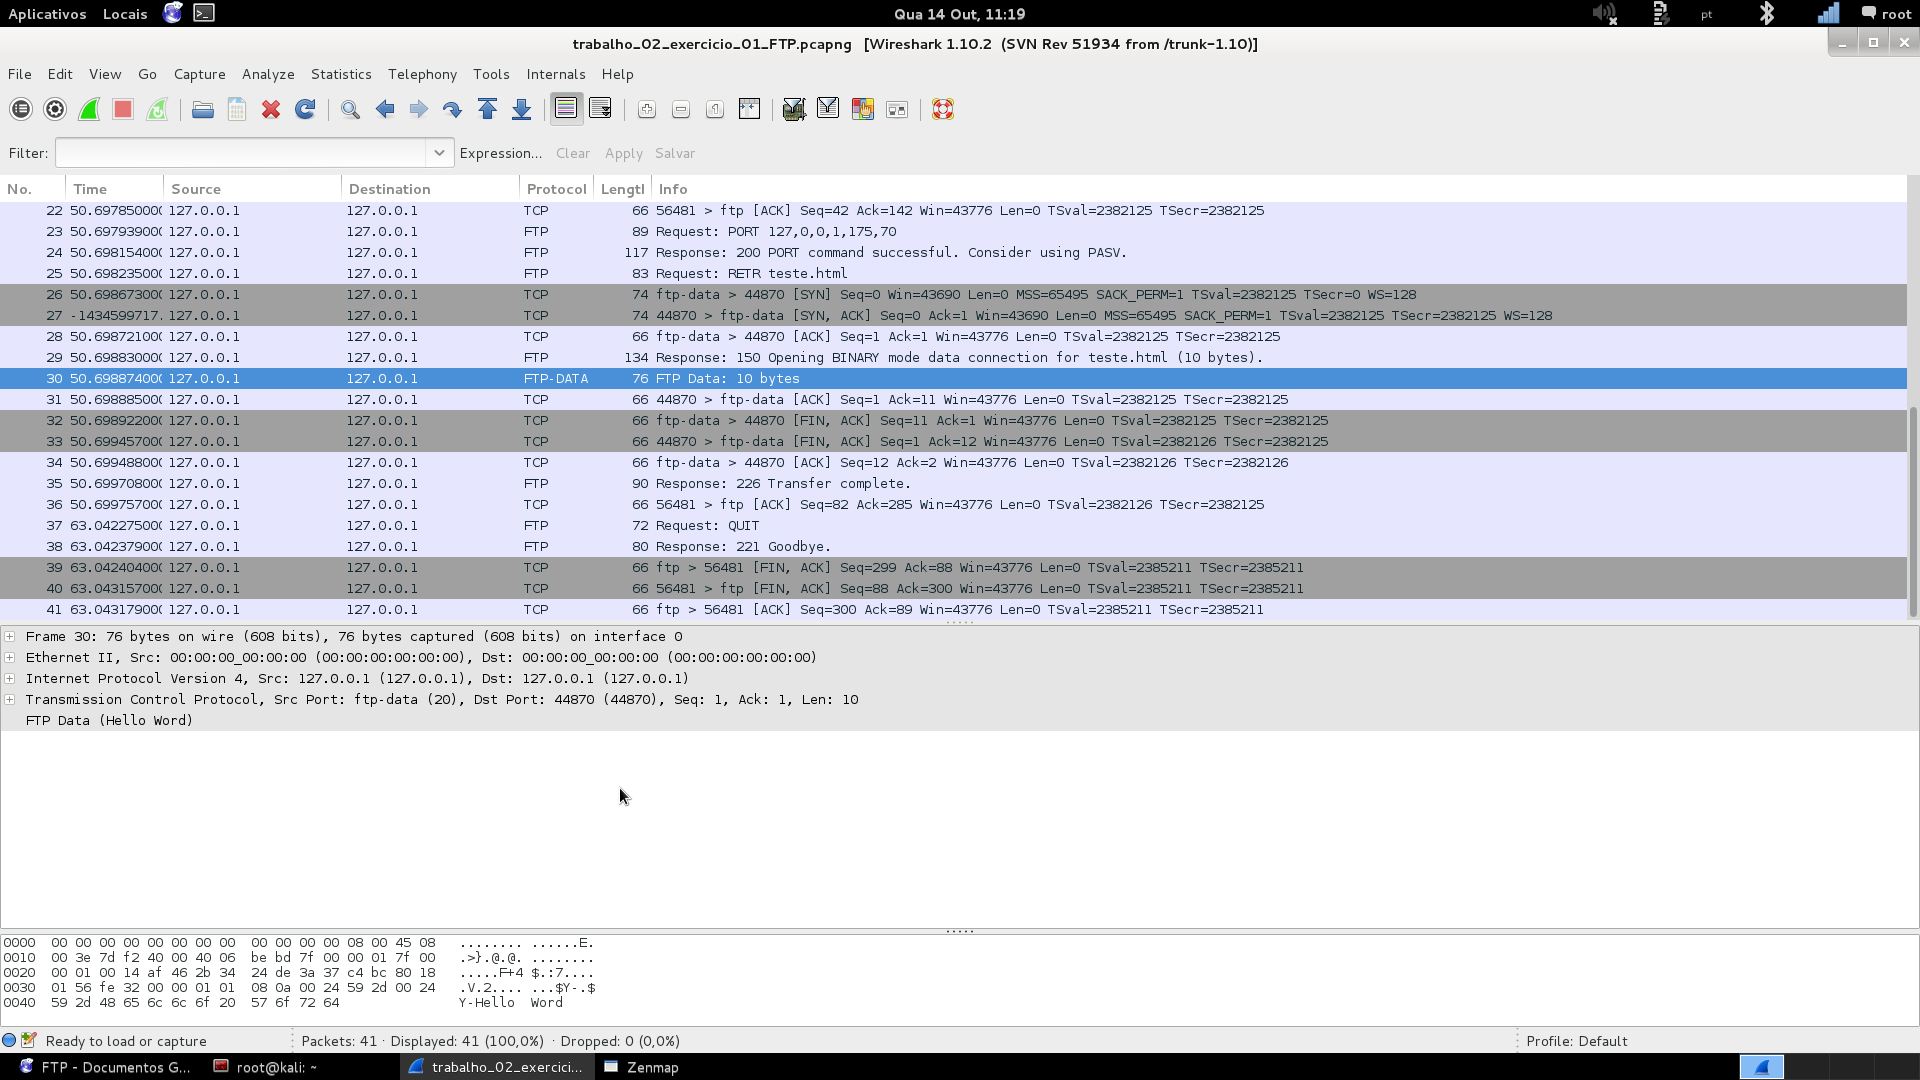
\includegraphics[width=450px, scale=1]{figuras/ftp2}
  \caption{Conexão TCP aberta para receber o FTP-Data}

\label{fig:ftp2}
\end{figure}

O TCP abre novamente o mesmo processo de conexão tree way handshake e ao final abre
uma conexão de dados (FTP-data) para enviar o arquivo. O arquivo é recebido com o conteúdo
"Hello Word" e a nova
conexão TCP é finalizada, de acordo com o ilustrado na Figura \ref{ref:ftp2}.

\subsection{Capturas de Encerramento}
Logo após receber a mensagem do cliente  contendo a mensagem QUIT, a conexão pode ser encerrada.
 Esse processo é iniciado quando o cliente envia um ACK, com número de Seq=299, para o servidor
  quando recebe o payload da requisição executada.

Logo quando este chega ao servidor, ele envia uma flag FIN, com Seq = 88, sinalizando o início
 da conversa para finalizar a conexão e um ACK = 300, sinalizando que recebeu o último
  pacote do cliente.

O cliente responde o servidor, confirmando o seu pedido de finalização com ACK = 300 e
também executa o pedido de FIN, com seq = 88.

Terminando a conexão, o servidor emitiu a confirmação do pedido de finalização com o ACK = 89.

\section{Protocolo DNS}

A captura de pacotes foi procedida no Sistema operacional Elementary OS 0.3.1 Freya

Foi utilizado o servidor local de DNS e a ferramenta de captura utilizada foi Wireshark  configurado para analisar os pacotes da interface wlan0.

\begin{itemize}

    \item Protocolo de Transporte Utilizado: UDP

    \item Endereço de IP e porta do Cliente: 172.16.5.158: 13706 

    \item Endereço de IP e porta do Servidor: 172.16.5.1: 53

\end{itemize}

\subsection{Conexão DNS}
Na Figura \ref{fig:http} , pode ser observado que o pacote de número 7 realiza um requisição informando o id da transação: 0x0e51, o tipo do servidor: A e por ultimo uma query com o domínio no qual ele deseja obter o endereço de IP: matriculaweb.unb.br. 


  \begin{figure}[h]
    \centering

    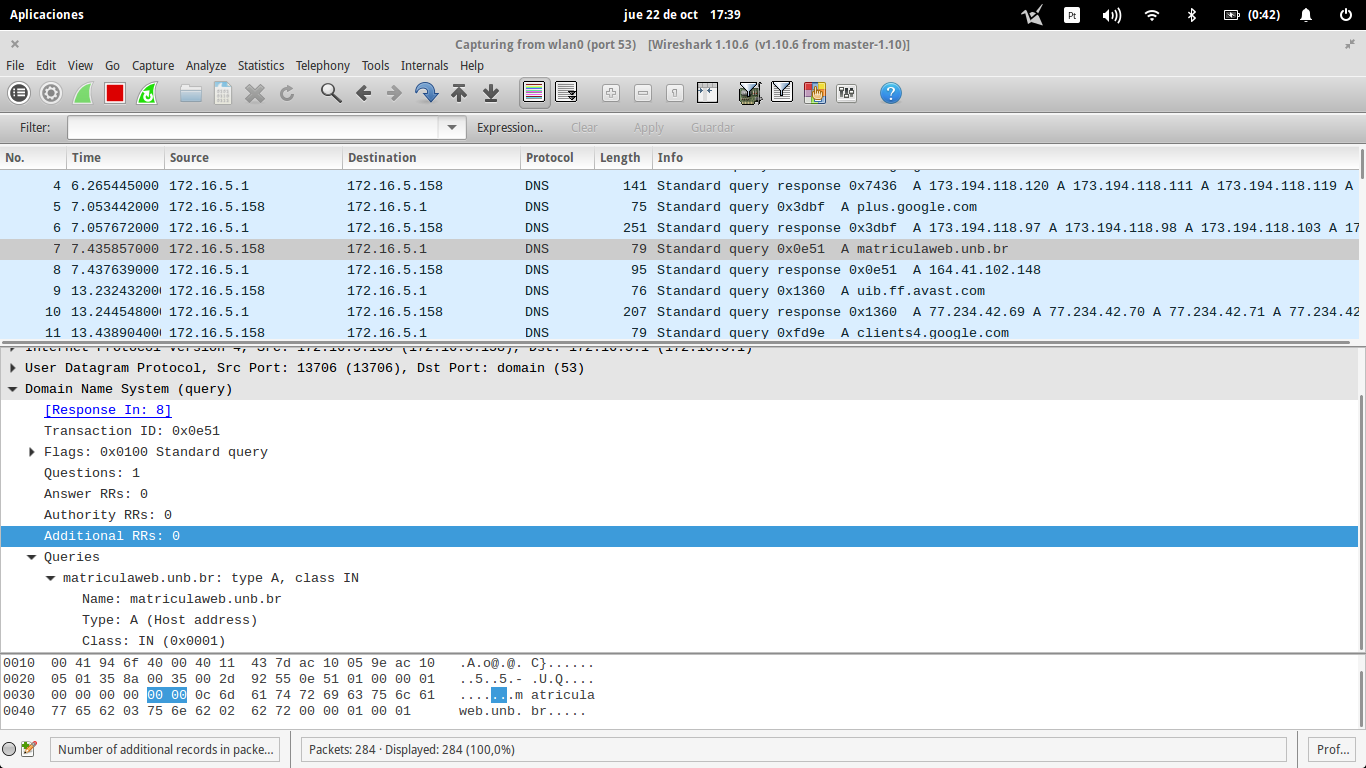
\includegraphics[width=450px, scale=1]{figuras/dns}
    \caption{Capturas de Pacotes em uma transação DNS}

 \label{fig:dns}
  \end{figure}

O pacote seguinte contém a resposta para a requisição. Ele informa o endereço de IP 164.41.102.148 correspondente ao domínio.

\section{Protocolo UDP}

A captura de pacotes foi procedida no Sistema operacional Elementary OS 0.3.1 Freya.

Realizou-se uma conexão UDP no servidor local. A ferramenta de captura utilizada foi Wireshark analisando os pacotes da interface wlan0.

\begin{itemize}

    \item Protocolo de Transporte Utilizado: UDP

    \item Endereço de IP e porta do Cliente: 192.168.25.47: 57621 

    \item Endereço de IP e porta do Servidor: broadcast: 57621

\end{itemize}



\subsection{Conexão UDP}
Na Figura \ref{fig:http}, observa-se uma conexão UDP. O pacote  de número 2371  possui em seu cabeçado os endereços da porta de origem e destino.

  \begin{figure}[h]
    \centering

    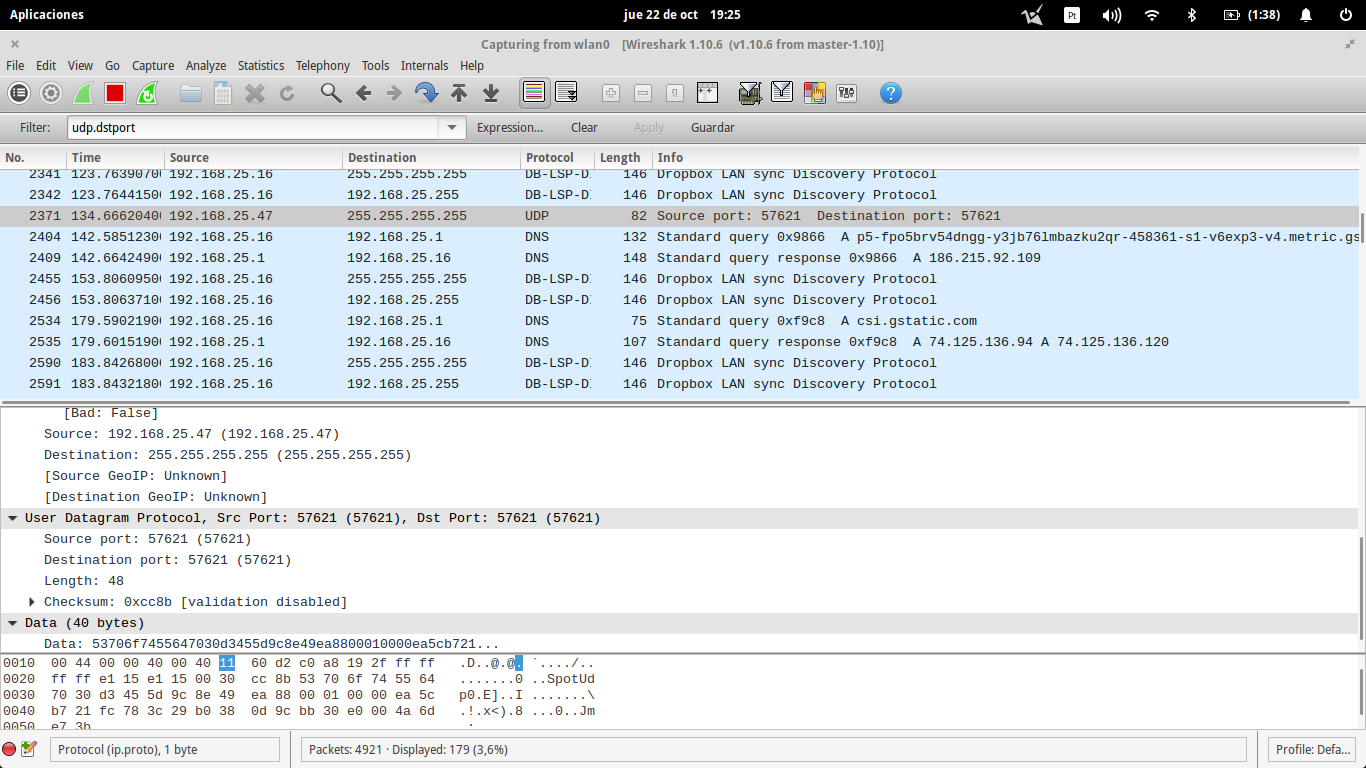
\includegraphics[width=450px, scale=1]{figuras/udp}
    \caption{Capturas de Pacotes em uma transação UDP}

 \label{fig:dns}
  \end{figure}